\graphicspath{{chapters/_resources/}}

\chapter{Journal Clubs}

\section{Enhancers are activated by p300/CBP activity-dependent PIC assembly, RNAPII recruitment, and pause release}

E1A binding protein p300/CREB-binding protein is a \emph{transcriptional co-activator} and \emph{histone acetyltransferase}. p300/CBP activity has been directly implicated in enhancer activation through acetylation (H3K27ac hallmark). p300/CBP-catalyzed acetylation promotes the recruitment of BRD4, and therefore the release of promoter-proximal-paused RNAPII. p300/CBP can regulate pro-proliferative pathways.

The aim of this article is to investigate the function and mechanisms of p300/CBP-catalyzed acetylation in dynamic enhancer activation.

To investigate the effects of p300/CBP inhibition on enhancers, SILAC (Stable isotope labeling by amino acids in cell culture) can be performed to obtain a relative quantification of A-485-induced acetylome and proteome changes. A-485 is a highly selective inhibitor of p300/CBP catalytic activity. 

Time-resolved nascent transcription analyses in A-485-treated ESCs [5-ethynyluridine sequencing (EU-Seq)] revealed that p300/CBP inhibition causes rapid enhancer deactivation. In addition, p300/CBP inhibition selectively downregulates cell-type-specific (CTS) genes.

TSA, a KDAC inhibitor, is able to fully recover acetylation levels after inhibition. TSA-induced transcription changes are not affected by A-485 co-treatment.

p300/CBP inhibition does not impair TF and p300 binding:
\begin{itemize}
\item increased p300 binding at TSS inversely correlates with reduced expression of downstream genes
\item p300/CBP activity appears to contribute to its dynamic dissociation from chromatin
\item chromatin binding of TFs and p300/CBP per se is not sufficient to activate enhancers
\end{itemize}

To investigate whether A-485-induced transcription inhibition results from a change in chromatin accessibility, ATAC-Seq can be applied to detect chromatin accessibility levels. It was observed that p300/CBP inhibition reduces chromatin accessibility, hence p300/CBP-catalyzed acetylation and/or ongoing transcription likely contributes to chromatin accessibility and rapid transcription inhibition by A-485 is unlikely due to a direct consequence of altered chromatin accessibility.

p300/CBP functions through BET-BRD-dependent and -independent mechanisms, BET inhibitors e.g. JQ1 slightly downregulate A-485 genes, but not as much as A-485. Indeed, p300/CBP activity promotes RNAPII recruitment independently of promoting pause release independently from BRD4.

p300/CBP-catalyzed acetylation promotes TFIID binding and PIC assembly:
\begin{itemize}
\item genes showing a slow TBP and RNAPII dissociation kinetics, such as Scl2a3 and Tfcp2l1, contain
TATA-box
\item genes displaying rapid TBP and RNAPII dissociation such as Nanog, Zfp42 and Esrrb, lack
canonical TATA-box
\item p300/CBP activity regulates the PIC assembly of enhancer-regulated, but not housekeeping genes.
\item reduction in TAF1, TBP and RNAPII binding is positively correlated
\end{itemize}

p300/CBP-catalyzed acetylation is crucial for TFIID anchoring, and, consequently, for PIC assembly and transcription initiation at enhancers and enhancer-regulated genes.

\textbf{Conclusions}
\begin{itemize}
\item p300/CBP and deacetylase activities regulate dynamic (de) activation of enhancers
\item p300/CBP-catalyzed acetylation promotes PIC assembly and RNAPII recruitment
\item BRD4 acts as a p300/CBP downstream effector to promote RNAPII pause release
\item Coupling of RNAPII recruitment and pause release enables rapid enhancer activation
\end{itemize}

\begin{figure}
\centering
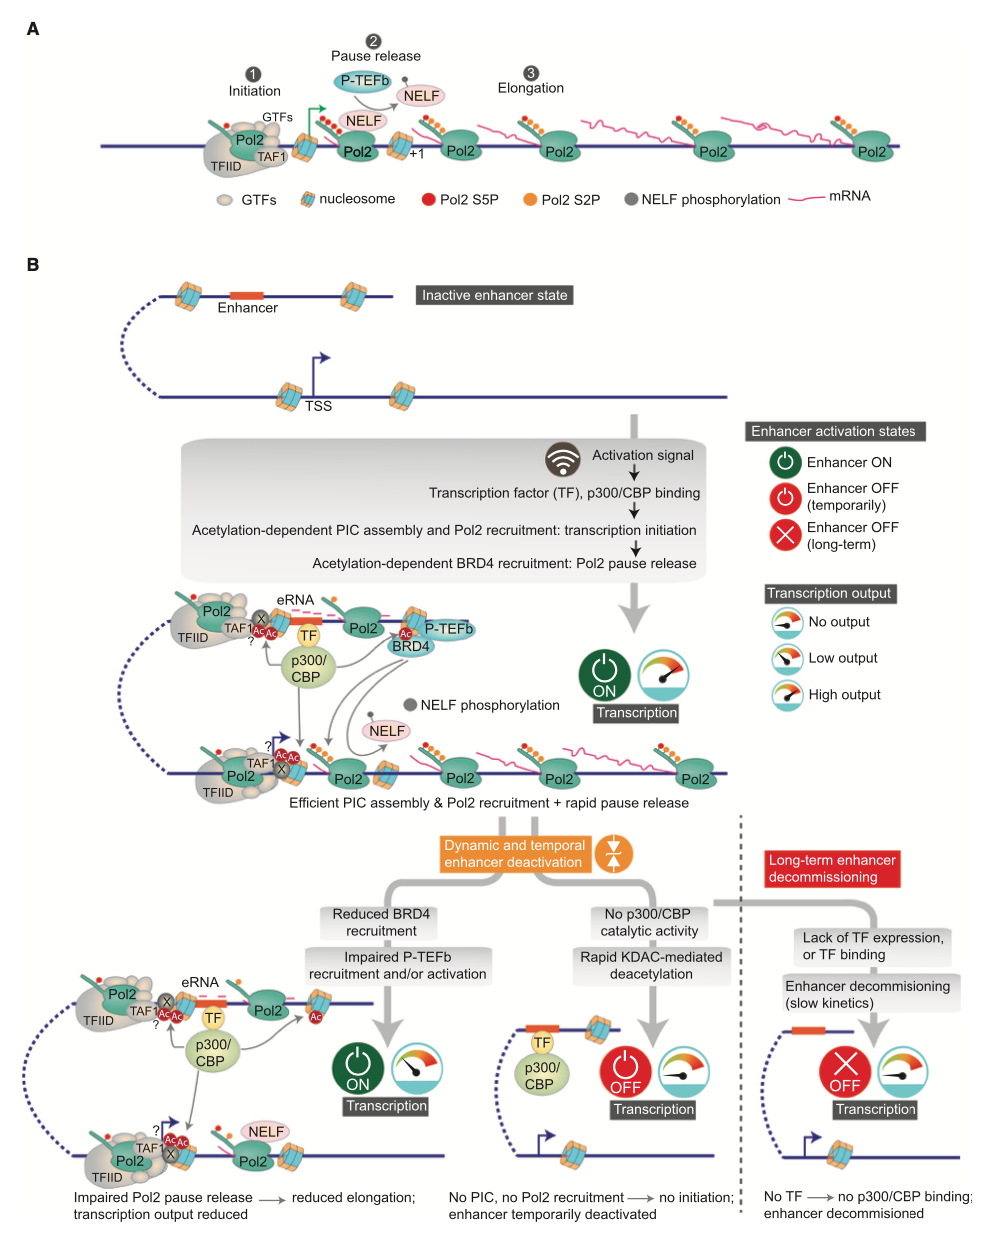
\includegraphics[width=\textwidth]{../_resources/Screenshot_2022-12-19_at_16-39-14.png}
\caption{(A) Schematic depiction of the key steps in the transcription cycle.
(B) Proposed hypothetical model of p300/CBP-activity-dependent dynamic enhancer activation. In response to activating signals, TFs recruit p300/CBP at enhancers where it acetylates chromatin-associated proteins. The acetylation of histones or non-histone proteins (X) promotes TFIID and RNAPII (Pol2) recruitment and transcription initiation. The question mark indicates the uncertainty of whether acetylation recruits TFIID directly or indirectly. Concurrently with promoting PIC assembly, p300/CBP-catalyzed acetylation promotes BRD4 binding, which facilitates Pol2 pause release by recruiting or activating P-TEFb. If BRD4 recruitment is impaired, then it leads to impaired Pol2 pause release and reduced transcription output. However, under this condition, p300/CBP continues to promote Pol2 recruitment, resulting in promoter proximal Pol2 pausing. If p300/CBP activity is inhibited, then PIC assembly, Pol2 recruitment, and pause release are impaired, leading to severe transcription inhibition. Under the conditions in which p300/CBP activity is impaired transiently, TFs and p300/CBP remain bound to chromatin and enhancers remain poised for rapid reactivation. However, if p300/CBP activity is inhibited for prolonged periods, then it will lead to reduced TF expression, which in turn will lead to impaired p300/CBP binding and long-term enhancer decommissioning.}
\end{figure}

\section{SPT5 stabilization of promoter - proximal RNA polymerase II}
Aoi et al. find that the conserved transcription elongation factor SPT5 stabilizes RNA polymerase II (RNA Pol II) in yeast and human
cells. SPT5 loss triggers degradation of a RNA Pol II subunit through CUL3, VCP, and CDK9. Stabilizing RNA Pol II may be a SPT5’s primary function to safeguard accurate gene expression.

Acute depletion studies: RNAPolII undergoes a 2-step pausing at NELF and at the +1 nucleosome: a depletion of NELF causes the RNAPolII to still be paused at the +1 nucleosome. Additional regulatory mechanism for the release of RNAPolII into the gene body.

SPT5 is an evolutionarily conserved and essential elongation factor. It forms the DSIF complex with SPT4. It interacts with RNAPolII throughout the elongation phase, probably active as a positive elongation factor, but impossible to knock-out.

Depletion of SPT5 through the generation of auxin-inducible degron (AID) avoids effects of long-term depletion and leads to an RBP1 degradation (the largest subunit of Pol II). 

SPT5 physically localizes with RNAPolII at most transcriptionally active genes on chromatin.Therefore, SPT5 depletion may affect the protein-protein interaction properties/composition of RNAPolII transcription units. \textbf{CUL3} is one of the human Cullin family proteins that serve as scaffolds of Cullin-RING E3 ubiquitin ligase complexes. Cul3 knockdown partially stabilized RBP1 upon SPT5 depletion, but did not affect SPT5-AID degradation. Recent studies showed how DNA damage causes RBP1 degradation by NEDD4 or CUL5, but upon SPT5 degradation they did not show any stabilization ability. CUL3- RNAPolII association on chromatin is triggered by SPT5-AID degradation.

\textbf{VPC} is known to mediate the unfolding of ubiquitylated proteins through its ATPase activity leading to efficient protein degradation.
VCP inhibition did not stabilize RBP1 when inhibiting initiation by triptolide (TPL).
There are (at least) two distinct pathways:
\begin{enumerate}
\item VCP-dependent degradation induced by SPT5 depletion
\item VCP-independent degradation induced by a TPL-stimulated initiation effect
\end{enumerate}
RBP1 is degraded either during the early elongation stage at promoter-proximal region, or during the productive elongation stage, in absence of SPT5.

To determine how SPT5 depletion and VCP inhibition affect the steady state of transcription by RNA Pol II, SPT5-AID cells were treated with the VCP inhibitor, followed by auxin, and then ChIP-seq for RNA Pol II was performed. RPB1 degradation induced by SPT5 loss occurs during the early stages of elongation. RNAPolII was able to travel substantial distances when SPT5 was depleted (although the distance was shorter than the control). RNAPolII at the elongation stage is unlikely to be degraded in the absence of SPT5. Even when RNAPolII is stabilized a the promoter-proximal region, it still needs SPT5 for the elongation stage in the body of the gene.

NELF regulates the transition of pausing states. Upon NELF loss, RNAPolII travels from a first pause region to a second pause region corresponding to the +1 nucleosome dyad. The SPT5 depletion system, coupled with the VCP inhibition described earlier, may allow us to precisely
investigate the SPT5 function in promoter-proximal pause/release. They performed precision run-on sequencing (PRO-seq) to map the RNA Pol II positions at base-pair resolution. RNA Pol II was paused at the second pause regions when depleting SPT5 and inhibiting VCP, which resembles NELF depletion.

\textbf{Conclusions}
SPT5 regulates promoter-proximal pausing at the first pause region, likely through its interaction with NELF, and that the transition to the second pause region upon SPT5 depletion is through NELF dissociating from RNA Pol II.
Two possible roles for SPT5:
\begin{enumerate}
\item SPT5 loss leads to unproductive elongation on nucleosomes, which may trigger RPB1 destabilization.
\item This raises another possibility: that SPT5 may regulate RPB1 stability and
proper elongation (pausing and velocity) independently.
\end{enumerate}

\begin{figure}
\centering
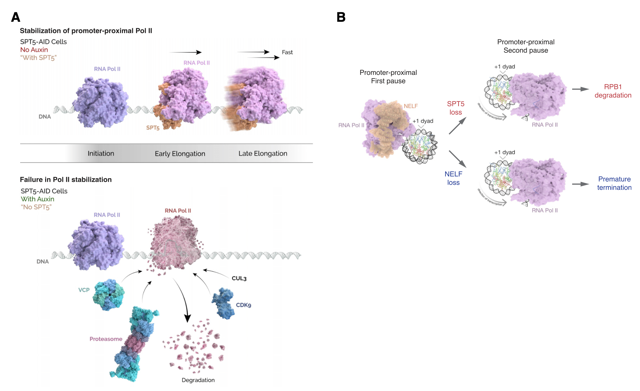
\includegraphics[width=\textwidth]{../_resources/Screen_Shot_2022-12-19_at_17-00-41.png}
\caption{(A) SPT5 stabilizes RNA Pol II during the early elongation stage. With the SPT5 protein (upper panel), once RNA Pol II is initiated and escapes from the promoter, RNA Pol II undergoes productive elongation until termination. Without SPT5 (lower panel), early-elongating RNA Pol II undergoes RPB1 degradation that is mediated by the CUL3 ubiquitin ligase, the VCP unfoldase, and a novel form of the P-TEFb component CDK9. Late-elongating RNA Pol II without SPT5 can persist in transcription at a slower speed.
(B) Failure in RNA Pol II passage on the +1 nucleosome leads to 2 distinct pathways to eliminate RNA Pol II from chromatin.}
\end{figure}


\hypertarget{myc-recruits-spt5-to-rna-polymerase-ii-to-promote-processive-transcription-elongation}{%
\section{MYC Recruits SPT5 to RNA Polymerase II to Promote Processive Transcription Elongation}\label{myc-recruits-spt5-to-rna-polymerase-ii-to-promote-processive-transcription-elongation}}

MYC encodes for a nuclear phosphoprotein and is involved in cell cycle progression, apoptosis and cellular transformation. It forms heterodimers with MAX and binds to E-box containing DNA and regulates expression of non-coding transcripts and mRNA expression by RNA pol II.

\begin{figure}
\centering
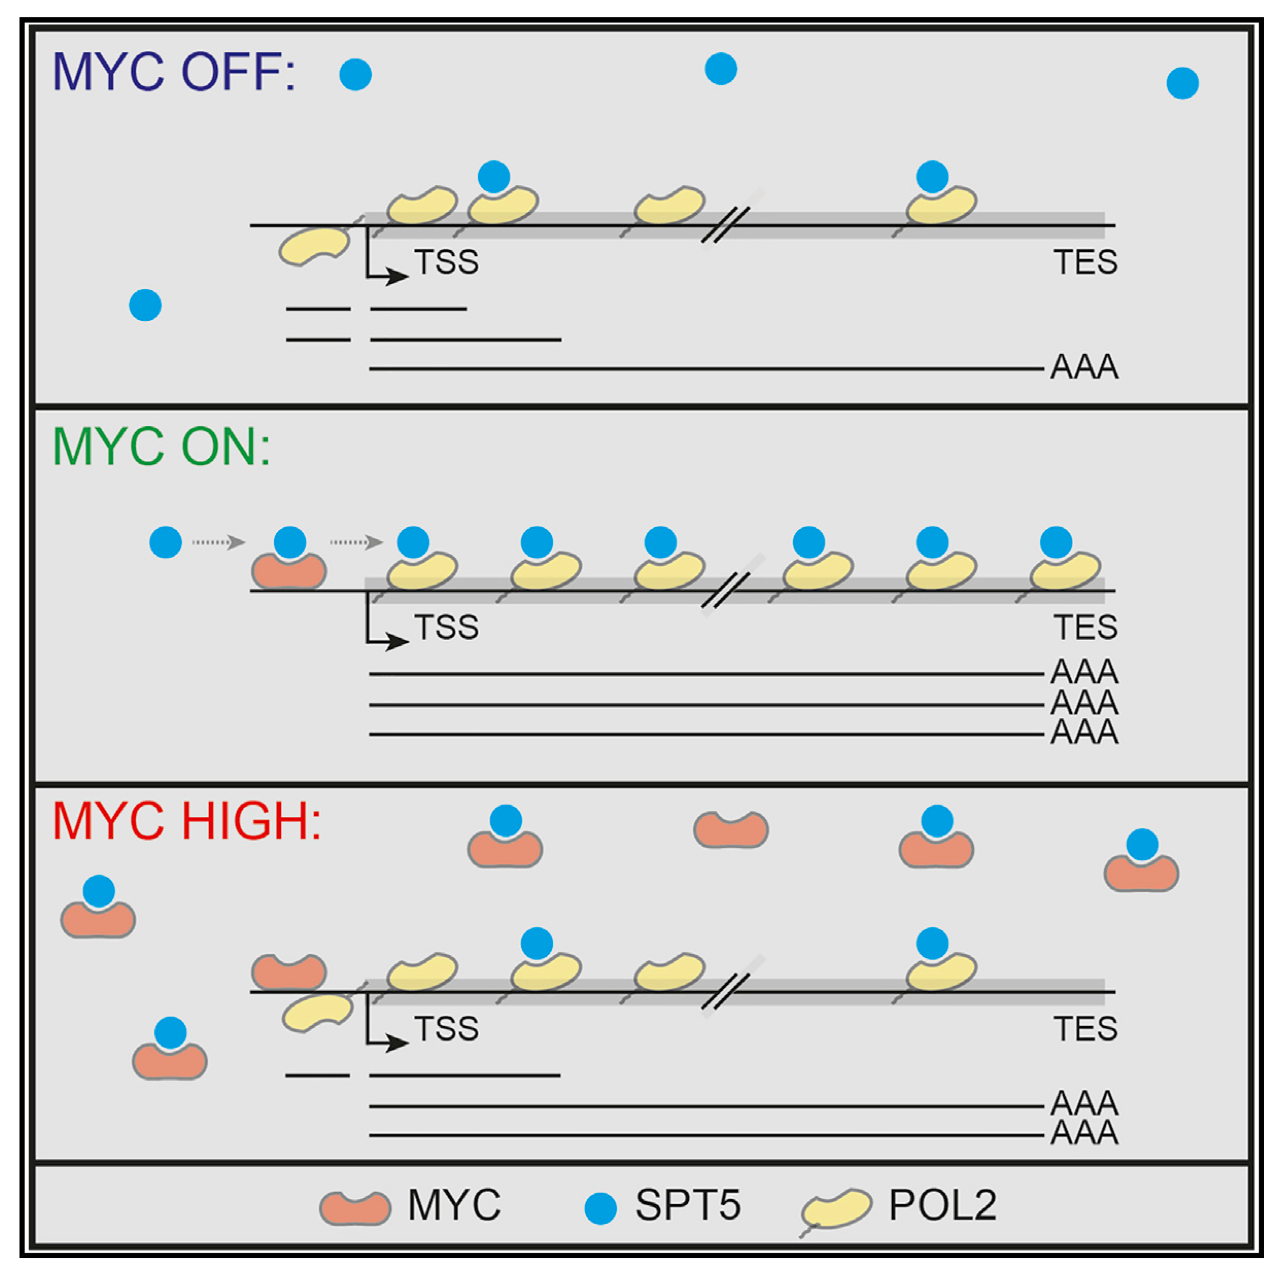
\includegraphics[width=0.5\textwidth]{../_resources/Screenshot_2022-10-28_at_10-37-23.png}
\caption{}
\end{figure}

ChiP-seq analysis revealed that MYC binds at the majority of open promoters. MYC is able to modulate the transcriptional cycle, and two mechanism are
proposed:

\begin{itemize}
\tightlist
\item
  MYC can recruit CDK9 to mediate pause release
\item
  MYC transfers Pol II associated factor PAF1 complex onto Pol II
\end{itemize}

Through the analysis of Tet-Off/On system, it was seen that MYC controls the assembly of transcriptionally engaged pol II complexes.
\begin{itemize}
\tightlist
\item
  6 common proteins in pol II and MYC interactome, but only SPT5 and SPT6 changed their association with Pol II upon MYC depletion
\item
  upon MYC depletion, read distribution at all expressed genes showed a
  global reduction of SPT5 binding → chromatin- associated Pol II binds
  to less SPT5 in the absence of MYC
\end{itemize}

By performing In situ Proximity Ligation Assay (PLA), we can achieve the detection of individual proteins or protein complexes using antibodies attached by DNA strands. PLA between SPT5 and pS2-Pol II shows clear reduction in nuclear proximity pair in absence of MYC in both U2OS and HMLE cells, meaning that upon MYC depletion we observe less interaction among SPT5 and Pol II. 

MYC recruits SPT5 by binding to its N-Terminal region.

CDK7 Activity is Required for Transfer of SPT5 from MYC to Pol II, as MYC facilitates the CDK7-dependent assembly of Pol II-SPT5 complexes.
In addition, MYC Influences Processivity and Directionality of Pol II after pause release:

\begin{itemize}
\tightlist
\item
  Reduced processivity and directionality upon MYC depletion
\item
  MYC Maintains High Pol II Elongation Rates
\item
  Overexpression of MYC has an inhibitory effect on Pol II elongation
  rate. SPT4 is sequestered by MYC, and therefore its binding with Pol
  II is decreased. Certain genes lose processivity and directionality at
  oncogenic levels of MYC → MYC dependent sequestration of SPT5 might
  repress tumor-suppressive genes.
\end{itemize}

MYC is not a pioneer TF, it only binds to accessible binding sites. MYC is able to bind low-affinity binding sites in a scenario of MYC overexpression.


\section{BRD4-directed super-enhancer organization of transcription repression programs links to chemotherapeutic efficacy in breast cancer}

BET are epigenetic leaders, they can recognize marks through
bromodomain. \textbf{BRD4} is a positive regulator of transcription. It
is involved in some disorders, as inflammation, obesity and cancer, as
it can enhance the transcription of oncogenes. JQ1 inhibits BET4 and is
a promising antitumor drug, but a resistance can be developed.

\textbf{Super-enhancers} are clusters of enhancers occupied by master
regulators e.g.~BRD4 or Mediator, which control the expression of
lineage-specific genes.

\begin{itemize}
\tightlist
\item
  NuRD complex: multi-subunit, repressor. Acts as chromatin remodeling
  complex and histone deacetylase.
\item
  LSD1: histone demethylase
\item
  Pellino (PEL1): E3 ubiquitin ligase
\end{itemize}

Thanks to MF we can identify interactors: all the components of LSD1/NuRD complex, confirmed
by Western Blotting and coIP assays.BRD4 is directly interacting with LSD1 through the C-terminus.


Interaction with factors known to reside in super-enhancer regions
e.g.~MED-1 was consolidated with ChIP-seq, almost 23000 targets in common.
The sequences bound are enriched in H3Kme1 and H3k27ac.

SE control genes in important signalling pathways and drug resistance e.g.~PDPK1.

After 4 weeks cancer resistant cells emerge. BRD4 is quickly inhibited,
while LSD1 or MTA3 in the early phase of treatment maintain chromatin
contact, which is exactly lost at 4 weeks.

\begin{enumerate}
\tightlist
\item
  removal of LSD1
\item
  increase of target genes expression
\item
  emergence of drug resistance
\end{enumerate}

BRD4 is required for LSD1/NuRD recruitment at super-enhancers

Reduced occupancy could be due to the lower protein levels: LSD1 mRNA
expression level is table upon JQ1 inhibition, but protein levels are
lower → proteosome action degrades the protein.

Elimination of PELI1 Improves the Therapeutic Efficacy of JQ1 in Breast Cancer Cells:
\begin{itemize}
\tightlist
\item
  Of 6 E3 ligases candidates, only PELI1 knockdown results in a strong
  increase of LSD1
\item
  PELI1 inhibition improves JQ1 therapeutic efficacy
\item
  the removal of BRD4/LSD1/NuRD complex from chromatin allows cancer
  cells to evade the selective pressure induced by JQ1 or other anti
  tumor drugs.
\end{itemize}

The Clinicopathological Significance of the
PELI1-LSD1-BRD4/LSD1/ NuRD Axis in Breast
Cancer:

\begin{itemize}
\tightlist
\item
  PELI1 mRNA levels are up-regulated when at least chemotherapy are
  applied
\item
  high expression of PELI1 leads to a worse survival rate
\end{itemize}

\begin{figure}
\centering
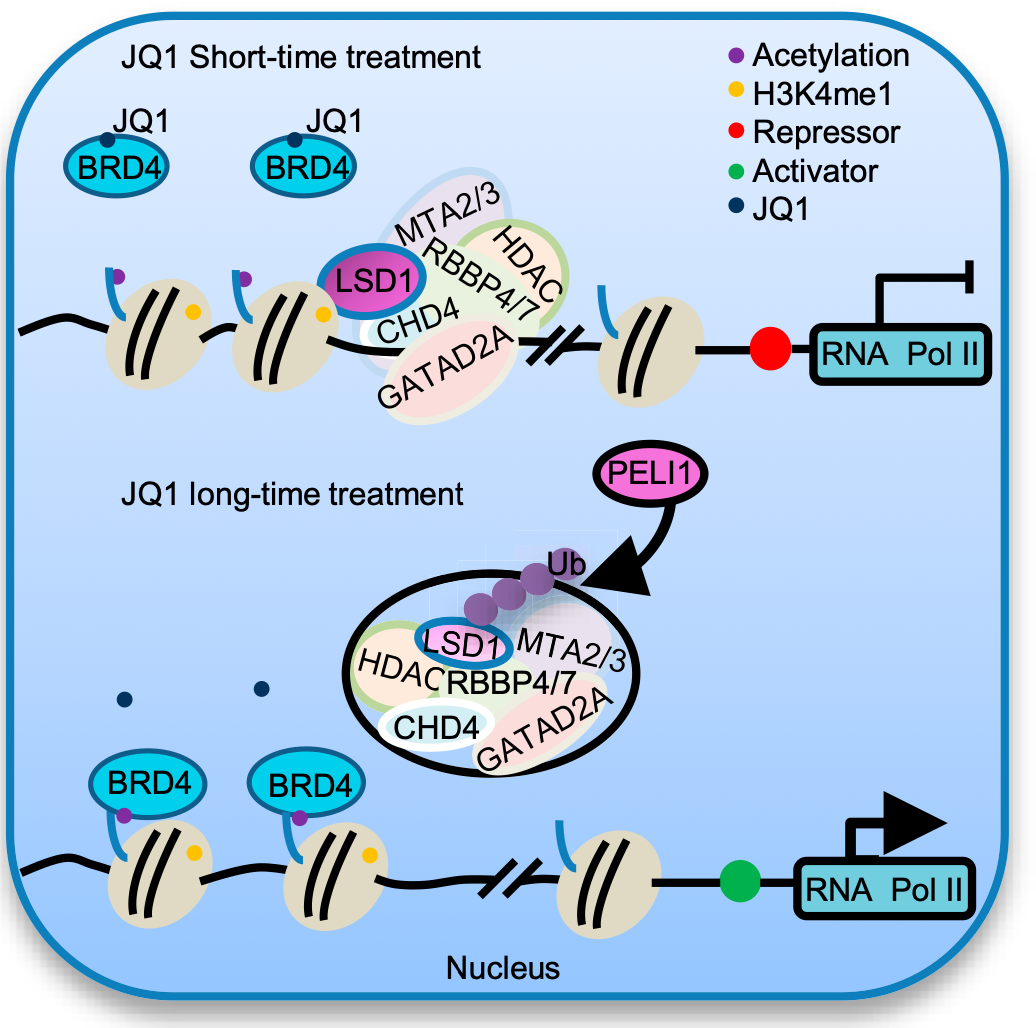
\includegraphics[width=0.5\textwidth]{../_resources/Screenshot_2022-10-28_at_11-55-04.png}
\caption{}
\end{figure}

Proposal: combined targeting of BRD4 and PELI1 as therapeutic for breast
cancer

\section{HSF2 cooperates with HSF1 to drive a transcriptional program critical for the malignant state}
c